\chapter{BlackFin architectuur}
	
	\section{BlackFin processor algemeen overzicht}

		\par De BlackFin processorfamilie is een 16- of 32-bit microprocessor ontwikkeld door het bedrijf Analog Devices. De processor beschikt over een ingebouwde fixed-point DSP die wordt bijgestaan door twee 16-bit MACs. Hiernaast is er in de chip ook nog een kleine processor aanwezig. De BlackFin processorreeks is ook ontwikkeld met het oogpunt op low power functionaliteiten.

		\par De BlackFin gebruikt een 32-bit RISC microcontroller die ge\"implementeerd is op een SIMD architectuur. Een BlackFin core bevat twee 16-bit hardware MACs, twee 40-bit ALUs en een 40-bit barrel shifter. Deze opstelling zorgt ervoor dat er maximaal drie instructies per klokcyclus uitgevoerd kunnen worden. Om het aantal instructies te reduceren zijn er ook vier DAGs ingebouwd in de processor.

		\par De BlackFin maakt gebruik van een byte-adresseerbare flat memory map. Het level 1 en level 2 geheugen is ingebouwd in de processor en het level 3 geheugen dient extern toegevoegd te worden. Al deze geheugens zijn gemapt op 32-bit adressen. Dit zorgt er voor dat de BlackFin processoren opgebouwd zijn volgens de Von Neumann architectuur.

		\par Het level 1 intern SRAM geheugen, dat geklokt is op de snelheid van de processor, is gebaseerd op de Harvard architectuur. Het instructie- en datageheugen is verbonden met de processor via een gereserveerde databus. Het level 2 geheugen is trager geklokt dan de processor zelf. De codememory kan zowel in level 1 als in level 2 geheugen opgeslagen worden.

		\par De BlackFin processor beschikt over twee DMA-controllers die kunnen opereren tussen de peripherals en de verschillende geheugens binnen de processor. Dankzij deze DMA-controllers wordt de processor niet belast met het uitvoeren van data transfers in het geheugen.

	\section{BlackFin BF-561 processor}

		\par De BlackFin BF-561 die aanwezig is op het EZ-KIT Lite beschikt over twee processorkernen. De processor kan werken op een kloksnelheid van maximaal 600 Mhz. Verder beschikt deze processor over 328 kB intern geheugen (level 1 en level 2).  Hiernaast beschikt de processor over twee 12-kanaals DMA controllers om de geheugen-naar-geheugen operaties uit te voeren. In figuur~\ref{fig:bf561fbd} is een overzicht van de opbouw van de BlackFin BF-561 weergegeven. 

			\begin{figure}[H]
				\centering
				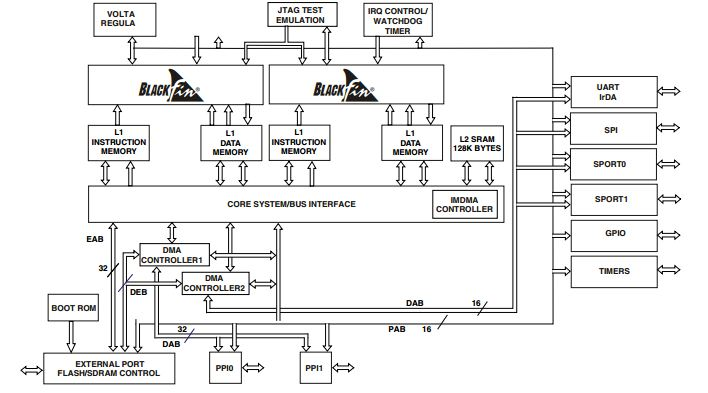
\includegraphics[width=0.95\textwidth]{Chapters/Chapter4/Images/bf-561.jpg}
				\caption{BF-561 functional block diagram}
				\label{fig:bf561fbd}
			\end{figure}

\chapter{Video Processing}

		%\par Er zijn verschillende mogelijkheden om video- en imageprocessing toe te passen met behulp van de BlackFin processoren. In de vlgende hoofdstukken worden drie van deze technieken kort omschreven. 
		
	\section{Interframe processing}
		
		\par Interframe processing wordt toegepast wanneer er een afhankelijk verband is tussen de verschillende frames. Dit is bijvoorbeeld het geval wanneer een inkomend frame vergeleken moet worden met een referentie frame. Het level 1 en 2 geheugen van de BlackFin processor zijn onvoldoende groot om deze frames in op te slaan. Er dient dus gebruik gemaakt te worden van het level 3 SDRAM. Het nadeel aan dit SDRAM geheugen is dat het veel trager is dan het ingebouwde level 1 en 2 geheugen van de processor zelf.  Een frame wordt onderverdeeld in verschillende delen die een sub block genoemd worden. Deze sub blocks worden vervolgens getransfereerd naar het level 1 geheugen van de BlackFinprocessor om verwerkt te worden. Indien het level 1 geheugen nog te klein blijkt te zijn kan het level 2 geheugen gebruikt worden als tussenbuffer. Alle geheugenoperaties worden uitgevoerd door de DMA-controller. In figuur~\ref{fig:interframe_processing} wordt een voorbeeld weergegeven van de hierboven beschreven techniek. Er bestaat een afhankelijkheid tussen currentframe en referenceframe.

			\begin{figure}[H]
				\centering
				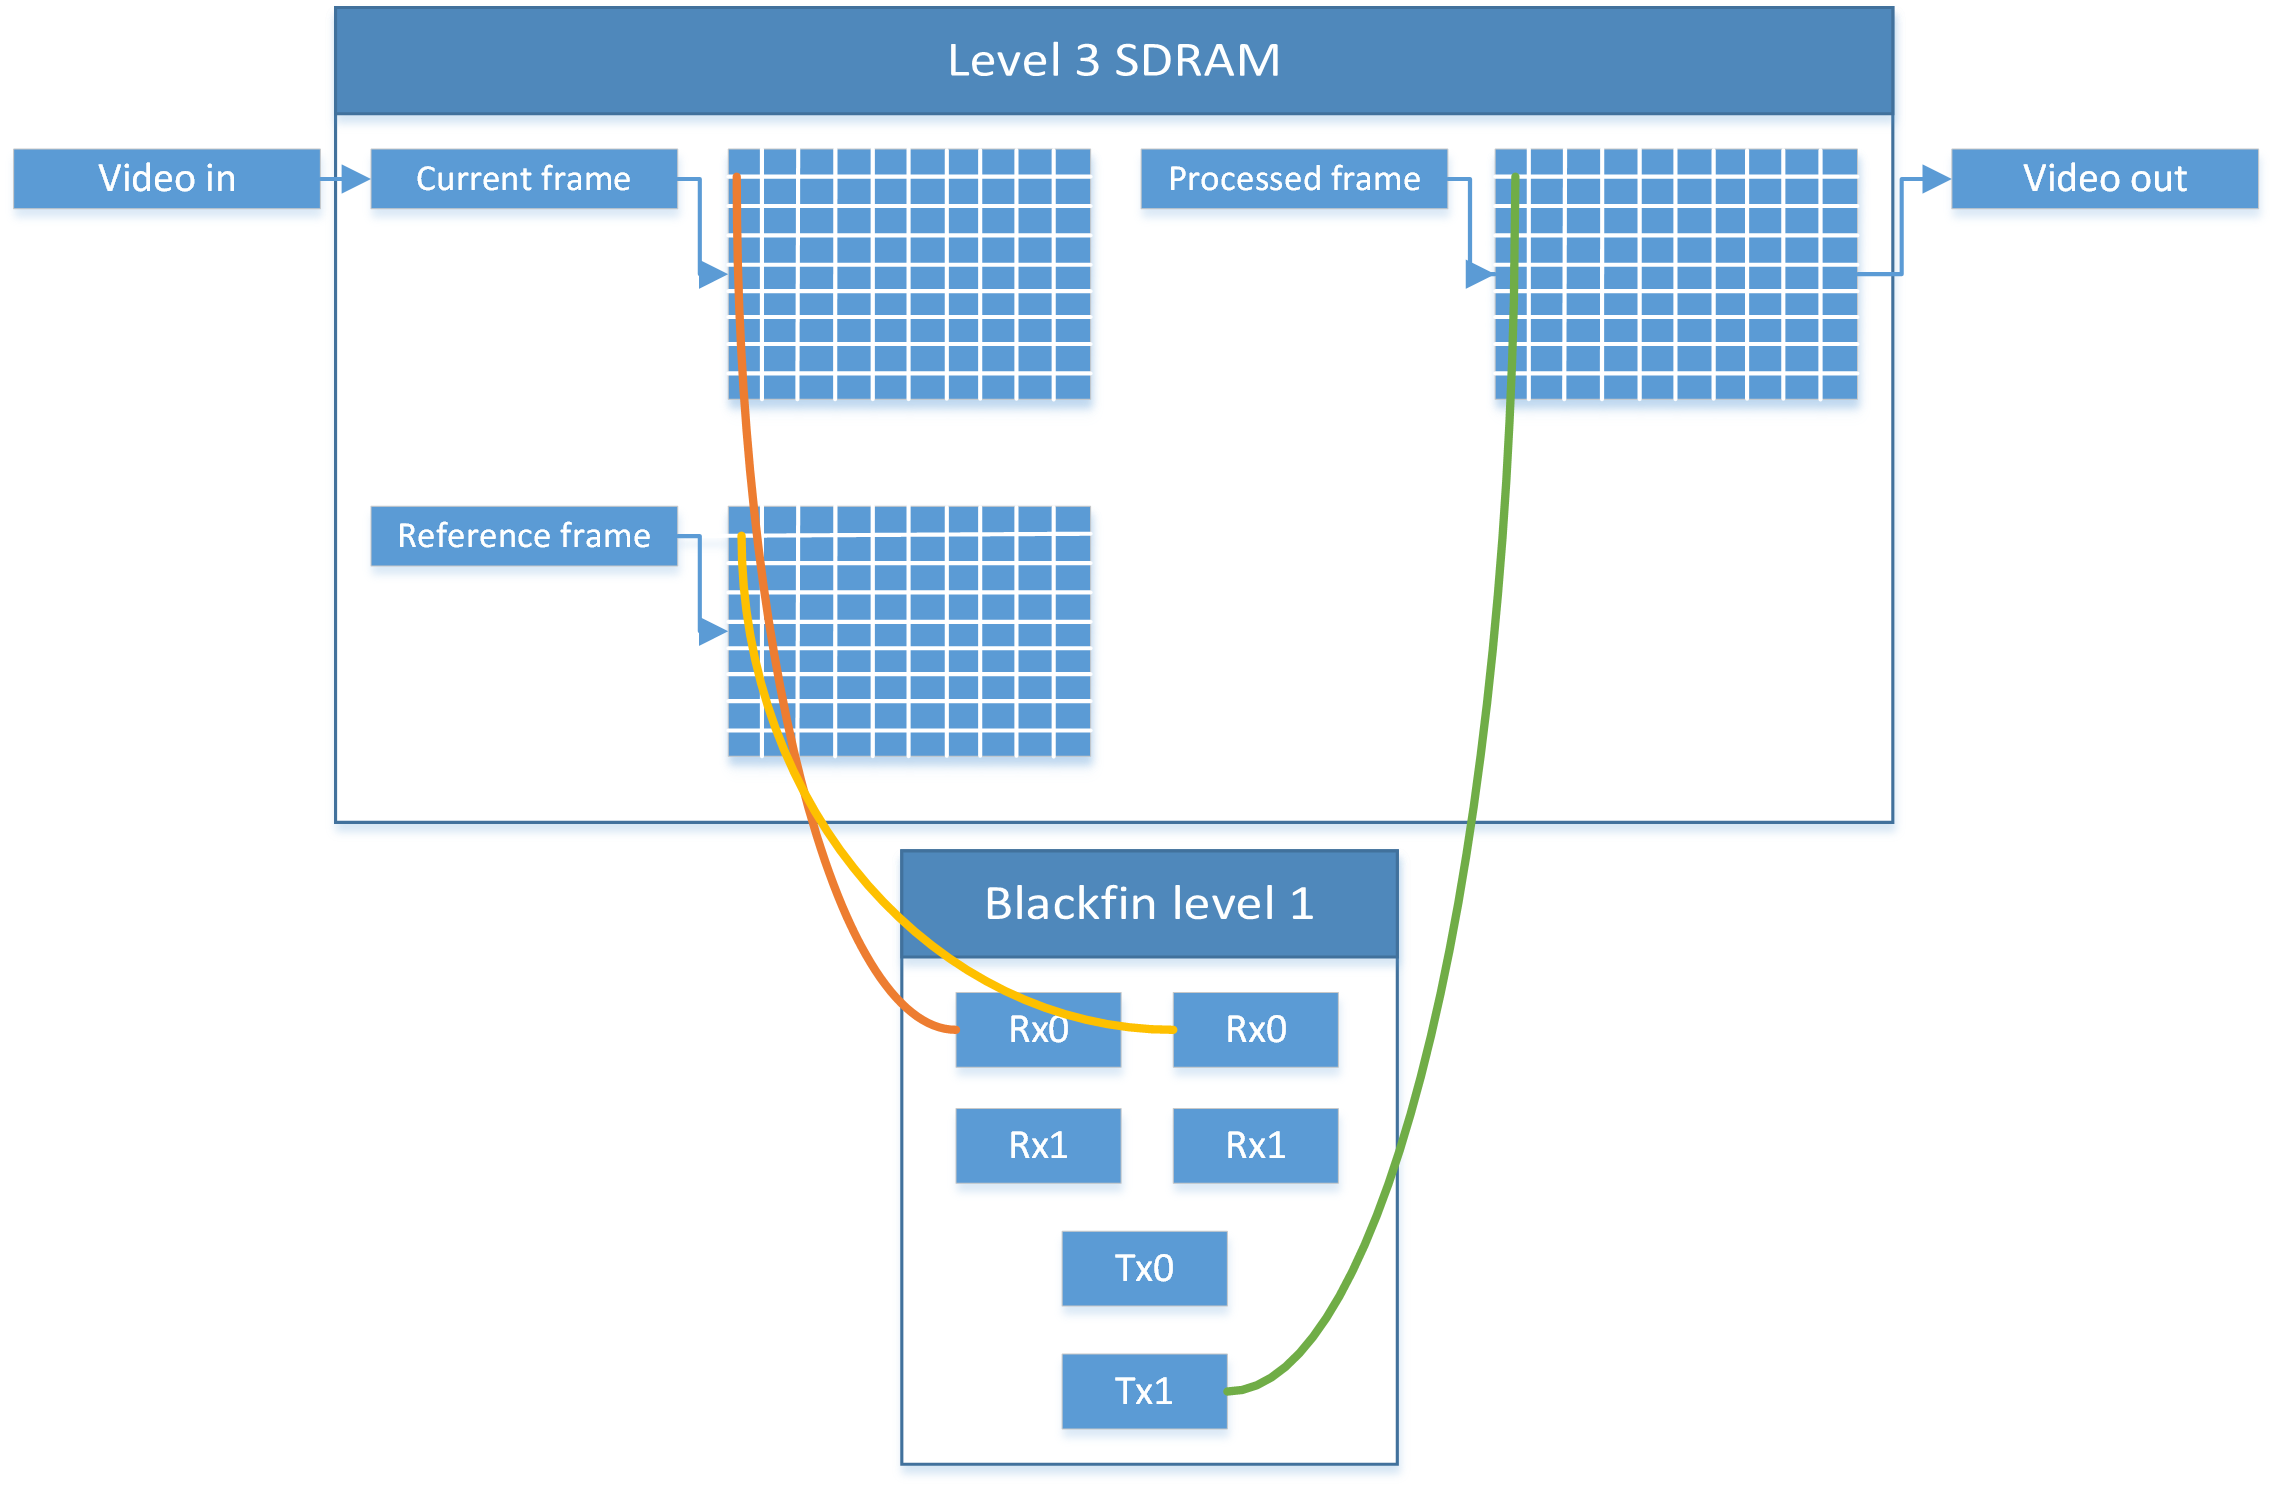
\includegraphics[width=0.90\textwidth]{Chapters/Chapter4/Images/DMA_interframe_processing.png}
				\caption{Interframe processing data flow diagram}
				\label{fig:interframe_processing}
			\end{figure}

	\section{Line processing}

		\par Bij het line processing principe wordt frame per frame te werk gegaan. Het frame zal in een eerste stap opgehaald worden uit het geheugen van de peripheral. Nadat een frame opgehaald is wordt het lijn per lijn verplaatst naar het level 1 geheugen van de BlackFin. Deze actie gebeurt door middel van de DMA-controller zodat de processor hier geen hinder van ondervindt.

		\par Een nog effici\"entere methode is om de data onmiddelijk van de peripheral lijn per lijn naar het level 1 geheugen te transfereren. Na der verwerking moet ook de data terug verstuurd worden naar een peripheral om deze weer te geven. Dit kan ook onmiddelijk lijn per lijn vanuit het level 1 geheugen, maar ook via het level 3 geheugen waar een volledig frame gebufferd kan worden. 

		\par In figuur~\ref{fig:line_processing} wordt de opbouw van een lijn-gebaseerde aanpak weergegeven. De DMA wordt gebruikt om data onmiddelijk naar het level 1 geheugen van de BlackFin te transfereren. Vervolgens wordt door de BlackFin een actie uigevoerd op de videolijn die dan weer wordt getransfereerd van het level 1 geheugen naar de video encoder. Deze transfers gebeuren door middel van de DMA-controlller. De dubbele buffering in het level 1 geheugen zorgt ervoor dat de DMA en de processing door de BlackFin processor concurrent uitgevoerd kunnen worden. Op deze manier kan video in realtime verwerkt worden.

			\begin{figure}[H]
				\centering
				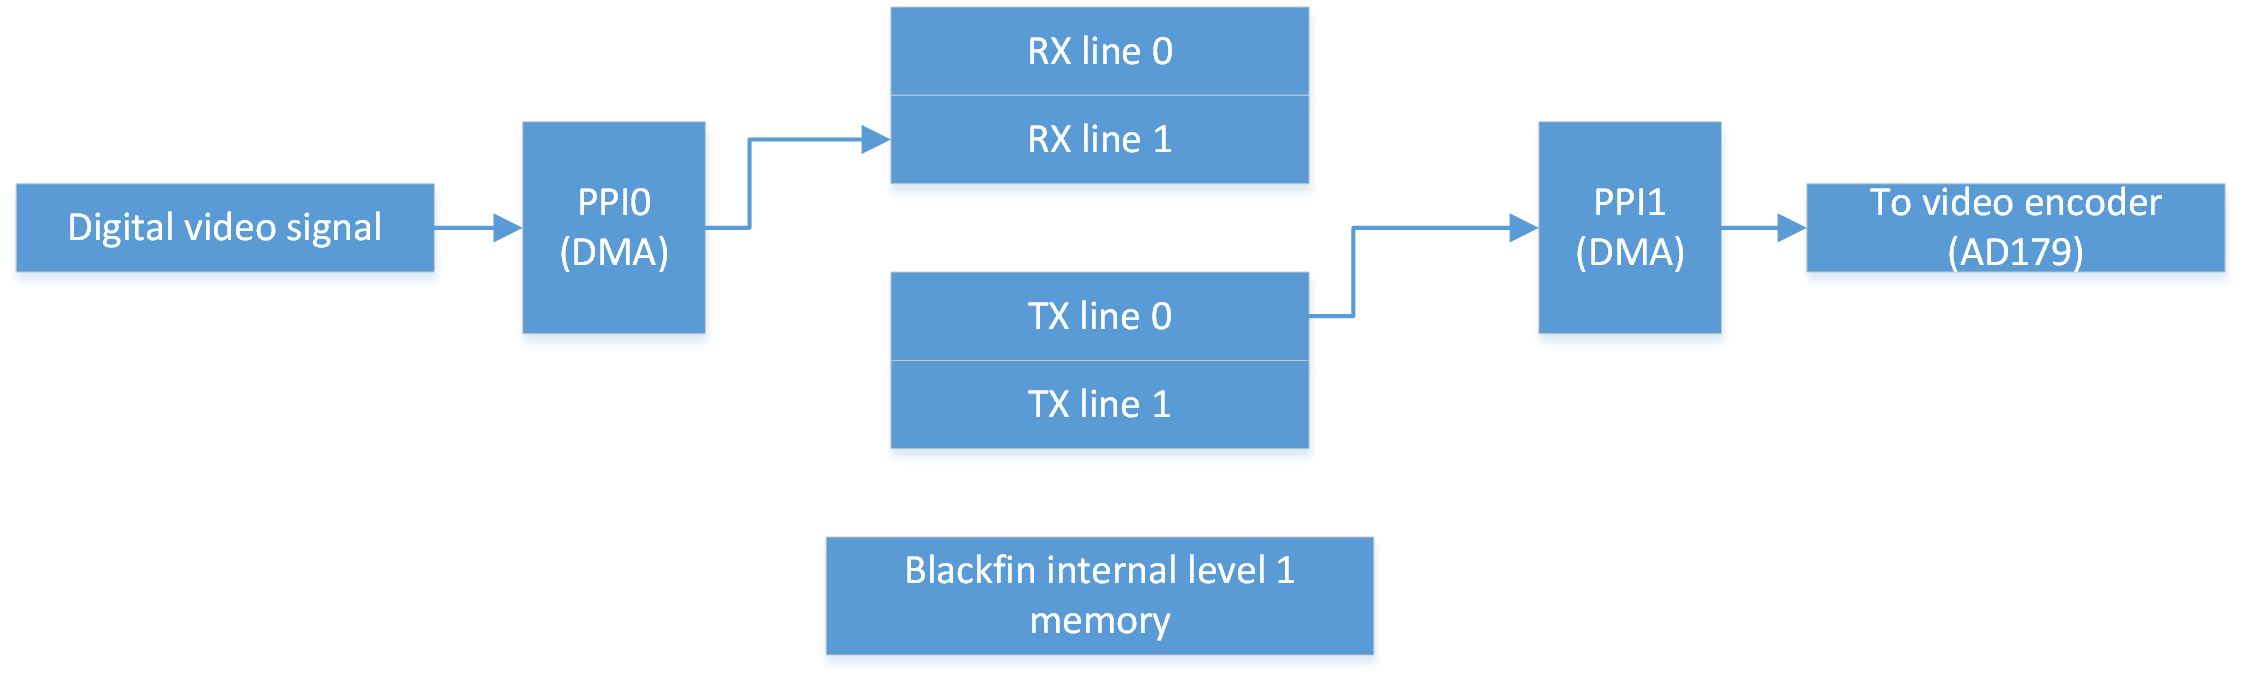
\includegraphics[width=0.95\textwidth]{Chapters/Chapter4/Images/DMA_line_processing.png}
				\caption{Line processing data flow diagram}
				\label{fig:line_processing}
			\end{figure}
	\newpage
	\section{Macro block processing}
		
		\par Bij macro block processing wordt het frame niet in zijn geheel verwerkt, maar opgedeeld in verschillende secties. Elke sectie heeft een dimensie van n bij m. De hoogte van de macroblock wordt weergegeven door n en de breedte door m. Het level 1 geheugen van de BlackFinprocessor is te klein om een alle n-lijnen van een afbeelding op te slaan, daarom wordt gebruik gemaakt van het level 2 geheugen. Dit zorgt ervoor dat er minder bandbreedte van de databus gebruikt wordt. 

		\par Ook bij het level 2 gheugen is de opslagcapaciteit beperkt. Een volledige afbeelding past vaak niet in het level 2 geheugen. Daarom wordt slechts een aantal lijnen van de afbeelding (n lijnen) in het level 2 geheugen geplaatst. Dit gebeurt door middel van de parallel peripheral interface van de DMA. Vervolgens zullen macroblocks verplaatst worden van het level 2 geheugen naar het level 1 geheugen waar deze verwerkt kunnen worden door de BlackFin processor. Er vindt een dubbele buffering plaats in zowel het level 1 als het level 2 geheugen. Telkens wordt de DMA-controller gebruikt voor deze geheugenoverdracht zodat de processor hier geen hinder van ondervindt.

		\par In figuur~\ref{fig:block_processing} is een voorbeeldopstelling te zien van macro block processing. In dit voorbeeld worden twee DMA-controllers gebruikt om de dataoverdrachten uit te voeren. Er wordt ook een dubbele framebuffering voorzien om de processwindow te vergroten.

			\begin{figure}[H]
				\centering
				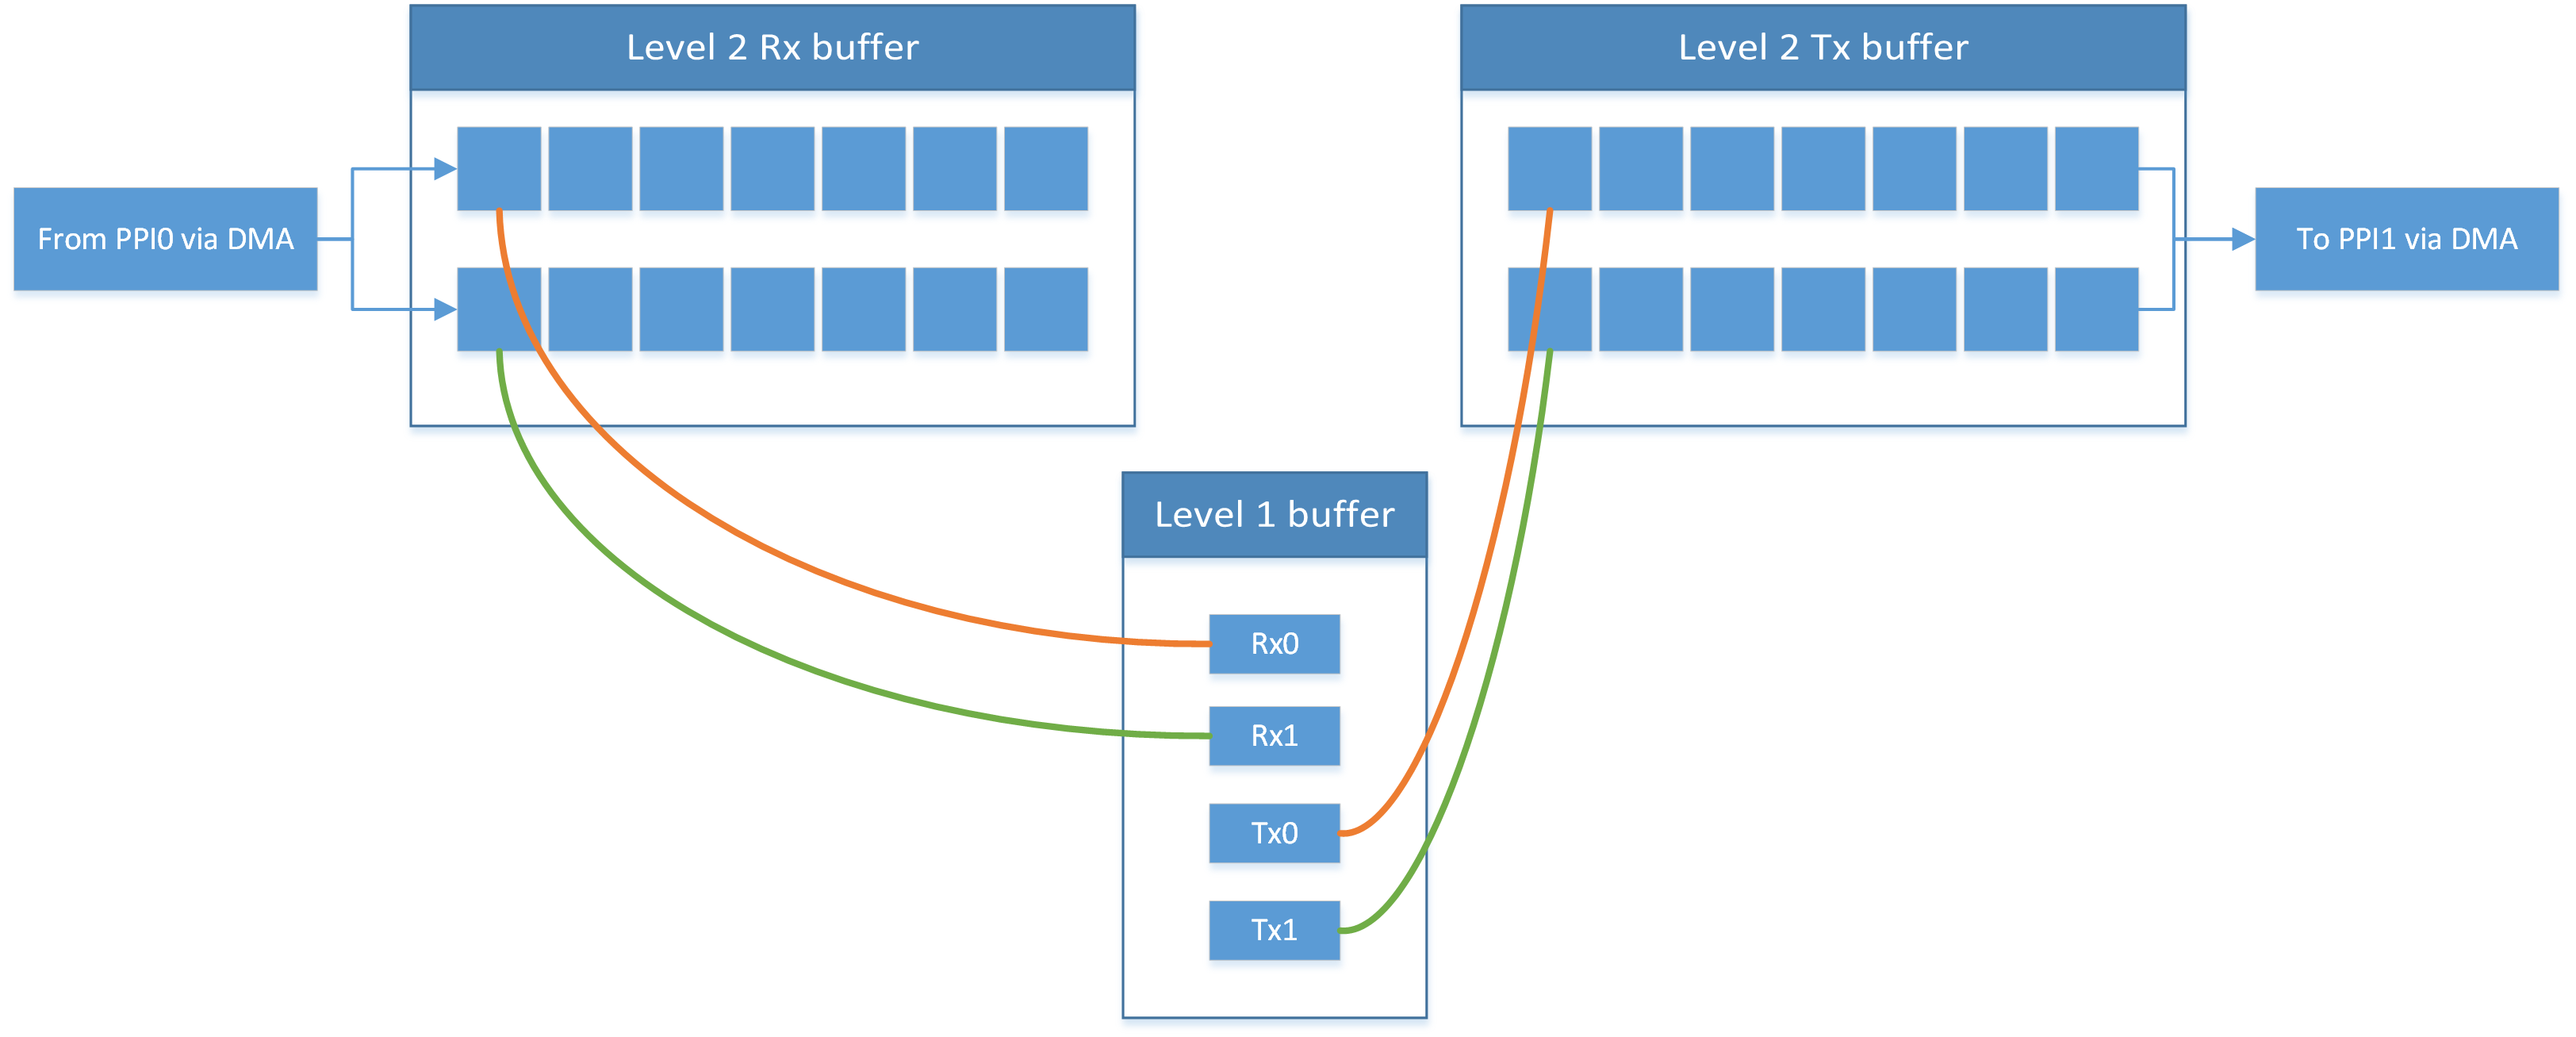
\includegraphics[width=0.95\textwidth]{Chapters/Chapter4/Images/DMA_block_matrix.png}
				\caption{Macro block processing data flow diagram}
				\label{fig:block_processing}
			\end{figure}
	\newpage
	\section{Optimalisatie}
		
		\par Door bij het design rekening te houden met de architectuur van de BlackFin processor kan er flink wat snelheid gewonnen worden. In de paragrafen hieronder worden enkele design tips kort toegelicht.

		\par Wanneer men via een DMA-controller data wil verplaatsen van het ene geheugen naar het andere geheugen dient men rekening de houden met de breedte van de data bus. Bij de BlackFin BF-56x reeks is er een 32-bit brede databus voorzien. Door de DMA-controller zo in te stellen dat hij per operatie telkens 32-bit of een veelvoud daarvan moet verplaatsen, wordt er optimaal gebruik gemaakt van de DMA en databus.

		\par Om de DMA-controllers effici\"ent te gebruiken dient men er rekening mee te houden bij het ontwerp dat nooit twee geheugentransferts plaatsvinden op het zelfde moment binnen eenzelfde DMA kanaal. 

		Bronnen:~\cite{bib_6},~\cite{bib_8},~\cite{bib_10},~\cite{bib_11}.


